\documentclass[a4paper,11pt]{article}

\usepackage[T1]{fontenc}
\usepackage[utf8]{inputenc}
\usepackage{tgpagella}
\usepackage{geometry}
\geometry{left=22mm,right=22mm,top=22mm,bottom=24mm}

\usepackage{xcolor}
\usepackage{graphicx}
\graphicspath{{figures/}{/output/figures/}{/Users/bd/Projects/thesis/output/figures/}}
\usepackage{booktabs}
\usepackage{array}
\usepackage{tabularx}
\usepackage{longtable}
\usepackage{enumitem}
\usepackage{amsmath,amssymb,mathtools}
\usepackage{tikz}
\usetikzlibrary{arrows.meta,positioning,calc,shapes.geometric,fit}
\usepackage{titlesec}
\usepackage{fancyhdr}
\usepackage{hyperref}
\usepackage{listings}
\usepackage{caption}

\definecolor{deepnavy}{HTML}{182337}
\definecolor{slate}{HTML}{34495E}
\definecolor{conceptFrame}{HTML}{1D4E89}
\definecolor{conceptBack}{HTML}{EAF3FF}
\definecolor{paperFrame}{HTML}{2D6A4F}
\definecolor{paperBack}{HTML}{EDF8F1}
\definecolor{codeFrame}{HTML}{465A69}
\definecolor{codeBack}{HTML}{F1F4F6}
\definecolor{researchFrame}{HTML}{6D3A9C}
\definecolor{researchBack}{HTML}{F4ECFA}
\definecolor{driftFrame}{HTML}{B23A2F}
\definecolor{driftBack}{HTML}{FFF1EA}

\hypersetup{
  colorlinks=true,
  linkcolor=conceptFrame,
  urlcolor=researchFrame,
  citecolor=conceptFrame,
  pdftitle={State-Based Process Monitoring Task Sheet},
  pdfauthor={RWTH Aachen PADS}
}

\titleformat{\section}
  {\Large\bfseries\color{deepnavy}}
  {\thesection}{0.7em}{}
\titleformat{\subsection}
  {\large\bfseries\color{slate}}
  {\thesubsection}{0.7em}{}
\titlespacing*{\section}{0pt}{2.4ex plus 0.4ex minus 0.2ex}{1.0ex}
\titlespacing*{\subsection}{0pt}{1.8ex plus 0.3ex minus 0.2ex}{0.8ex}

\pagestyle{fancy}
\fancyhf{}
\lhead{\small State-Based Process Monitoring}
\rhead{\small BSc Thesis Task Sheet}
\cfoot{\small \thepage}
\renewcommand{\headrulewidth}{0.4pt}
\renewcommand{\footrulewidth}{0pt}

\setlist[itemize]{leftmargin=1.4em,itemsep=0.25em,topsep=0.35em}
\setlist[enumerate]{leftmargin=1.6em,itemsep=0.25em,topsep=0.35em}
\renewcommand{\arraystretch}{1.18}
\newcolumntype{Y}{>{\raggedright\arraybackslash}X}
\newcolumntype{C}[1]{>{\centering\arraybackslash}p{#1}}

\lstdefinestyle{python}{
  language=Python,
  basicstyle=\ttfamily\footnotesize,
  keywordstyle=\color{conceptFrame}\bfseries,
  stringstyle=\color{paperFrame},
  commentstyle=\color{codeFrame}\itshape,
  numbers=left,
  numberstyle=\tiny\color{codeFrame},
  stepnumber=1,
  numbersep=6pt,
  showstringspaces=false,
  breaklines=true,
  frame=single,
  rulecolor=\color{codeFrame},
  backgroundcolor=\color{codeBack},
  columns=fullflexible,
  keepspaces=true
}

\newcounter{task}
\newcommand{\Task}[1]{%
  \refstepcounter{task}%
  \par\medskip
  \noindent{\large\bfseries Task \thetask: #1}\par\smallskip
}

\newcommand{\answerspace}[1][1.0cm]{\par\vspace{#1}}
\newcommand{\blankline}{\par\noindent\rule{\linewidth}{0.35pt}\par}
\newcommand{\vect}[1]{\boldsymbol{#1}}
\newcommand{\R}{\mathbb{R}}
\newcommand{\onehot}{\operatorname{onehot}}

\newcommand{\WindowTimeline}{%
\begin{center}
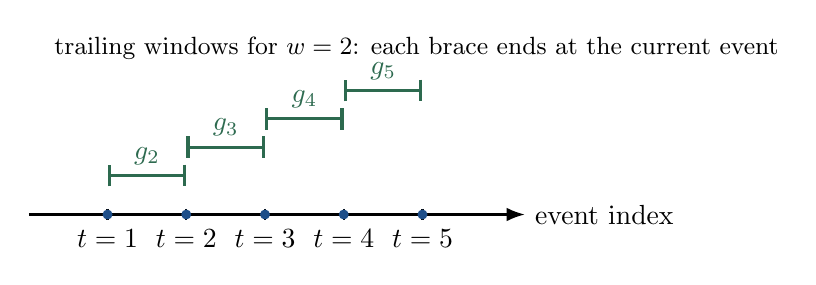
\begin{tikzpicture}[x=1.0cm,y=0.9cm,>=Latex]
  \draw[->,thick] (0,0) -- (6.3,0) node[right] {event index};
  \foreach \x/\lab in {1/1,2/2,3/3,4/4,5/5} {
    \draw[thick] (\x,0.08) -- (\x,-0.08);
    \node[below] at (\x,-0.08) {$t=\lab$};
    \fill[conceptFrame] (\x,0) circle (1.8pt);
  }
  \draw[paperFrame,very thick,|-|] (1,0.55) -- (2,0.55) node[midway,above] {$g_2$};
  \draw[paperFrame,very thick,|-|] (2,0.95) -- (3,0.95) node[midway,above] {$g_3$};
  \draw[paperFrame,very thick,|-|] (3,1.35) -- (4,1.35) node[midway,above] {$g_4$};
  \draw[paperFrame,very thick,|-|] (4,1.75) -- (5,1.75) node[midway,above] {$g_5$};
  \node[align=left,anchor=west] at (0.2,2.35) {\small trailing windows for $w=2$: each brace ends at the current event};
\end{tikzpicture}
\end{center}
}

\newcommand{\BlankSOMGrid}{%
\begin{center}
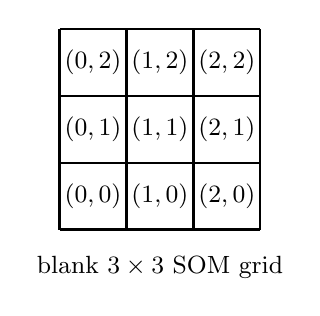
\begin{tikzpicture}[scale=0.85]
  \draw[step=1,thick] (0,0) grid (3,3);
  \foreach \x in {0,1,2} {
    \foreach \y in {0,1,2} {
      \node[font=\small] at (\x+0.5,\y+0.5) {$(\x,\y)$};
    }
  }
  \node[below] at (1.5,-0.25) {\small blank $3\times3$ SOM grid};
\end{tikzpicture}
\end{center}
}

\newcommand{\DriftTimeline}{%
\begin{center}
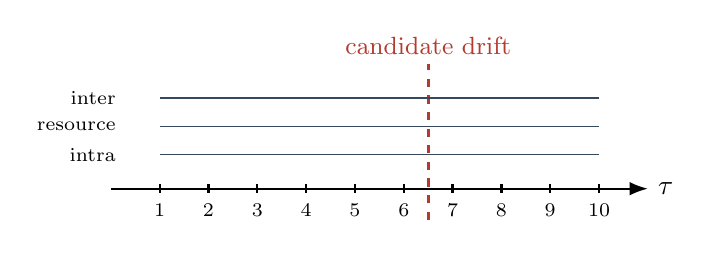
\begin{tikzpicture}[x=0.62cm,y=0.72cm,>=Latex]
  \draw[->,thick] (0,0) -- (11,0) node[right] {$\tau$};
  \foreach \x in {1,...,10} {
    \draw[thick] (\x,0.08) -- (\x,-0.08);
    \node[below,font=\scriptsize] at (\x,-0.1) {$\x$};
  }
  \draw[driftFrame,very thick,dashed] (6.5,-0.55) -- (6.5,2.2);
  \node[driftFrame,above,font=\small] at (6.5,2.2) {candidate drift};
  \foreach \row/\label in {0.6/intra,1.1/resource,1.6/inter} {
    \node[left,font=\scriptsize] at (0.3,\row) {\label};
    \draw[slate] (1,\row) -- (10,\row);
  }
\end{tikzpicture}
\end{center}
}

\begin{document}
\thispagestyle{empty}

\begin{center}
{\LARGE\bfseries State-Based Process Monitoring in Traditional Event Logs}
\end{center}

\tableofcontents
\newpage

\section{Paper Foundations}

\Task{Paper notation instantiations}
Use the tiny running example below to instantiate the paper notation. For each item (a)--(e), produce three outputs: a concrete instantiation using the example, the meaning of the instantiated object, and one short sentence about how it is used in the window--compress--map pipeline. Do not only define the symbols; write actual sets, maps, vectors, windows, or state assignments.

\begin{center}
\small
\begin{tabular}{c l l l l}
\toprule
Event & Activity & Time & Related objects & Attributes\\
\midrule
$e_1$ & Create & 08:00 & $\{o_1:\mathrm{Order},i_1:\mathrm{Item}\}$ & amount $=100$, channel $=\mathrm{web}$\\
$e_2$ & Ship & 09:00 & $\{o_1:\mathrm{Order},i_1:\mathrm{Item}\}$ & amount $=100$, channel $=\mathrm{web}$\\
$e_3$ & Create & 09:10 & $\{o_2:\mathrm{Order},i_2:\mathrm{Item},i_3:\mathrm{Item}\}$ & amount $=240$, channel $=\mathrm{phone}$\\
\bottomrule
\end{tabular}
\end{center}

Use, where needed, $A=\{\mathrm{Create},\mathrm{Ship}\}$, $OT=\{\mathrm{Order},\mathrm{Item}\}$, $K_{\mathrm{num}}=\{\mathrm{amount}\}$, and $K_{\mathrm{str}}=\{\mathrm{channel}\}$. For PCA and SOM, you may choose a small numerical example, but the numbers must be dimensionally consistent with the formulas.

\begin{enumerate}[label=(\alph*)]
\item \textbf{OCEL.} Let $U_\sigma$ denote the universe of all strings. An object-centric event log is
\[
(E,O,A,OT,\pi_{\mathrm{act}},\pi_{\mathrm{time}},\pi_{\mathrm{ot}},\pi_{\mathrm{omap}},
\pi_{\mathrm{vmap}},\pi_{\mathrm{ovmap}},\leq),
\]
where $E$ is the event set, $O$ the object set, $A$ the activity set, $OT$ the object-type set, and
\[
e_1 \leq e_2 \Longleftrightarrow \pi_{\mathrm{time}}(e_1)\leq \pi_{\mathrm{time}}(e_2)
\]
with tie-breaking for equal timestamps.
\item \textbf{Event encoding map.} For selected numeric and string event-attribute names $K_{\mathrm{num}}$ and $K_{\mathrm{str}}$,
\[
\begin{aligned}
x(e):={}&\left[
\onehot_A(\pi_{\mathrm{act}}(e)) \;\middle|\;
(c_t(e))_{t\in OT} \;\middle|\;
(v_k(e))_{k\in K_{\mathrm{num}}} \;\middle|\;\right.\\
&\left.\bigoplus_{k\in K_{\mathrm{str}}}
\onehot_{V_k\cup\{\operatorname{UNK}\}}(\pi_{\mathrm{vmap}}(e,k))
\right]\in\R^n,
\end{aligned}
\]
with
\[
c_t(e):=\left|\{o\in \pi_{\mathrm{omap}}(e):\pi_{\mathrm{ot}}(o)=t\}\right|\in\R_{\geq 0},
\quad
n:=|A|+|OT|+|K_{\mathrm{num}}|+\sum_{k\in K_{\mathrm{str}}}(|V_k|+1).
\]
\item \textbf{Per-object trailing window.} For object $o$ and sequence $x_{1:T}^{(o)}$,
\[
g_t^{(o)}:=\left[x_{t-w+1}^{(o)}\middle|x_{t-w+2}^{(o)}\middle|\cdots\middle|x_t^{(o)}\right]\in\R^{wn}.
\]
\item \textbf{PCA compression.} With centered data matrix $X_c\in\R^{m\times n}$,
\[
\Sigma:=\frac{1}{m}X_c^\top X_c,\qquad
\Sigma v_i=\lambda_i v_i,\qquad
z=W^\top(x-\mu),\qquad
\hat{x}=\mu+WW^\top(x-\mu).
\]
The explained variance ratio is
\[
\operatorname{EVR}(d):=\frac{\sum_{i=1}^{d}\lambda_i}{\sum_{i=1}^{n}\lambda_i}.
\]
\item \textbf{SOM BMU and boundary condition.} For SOM prototypes $w_i$ at grid coordinates $r_i$,
\[
b(x):=\arg\min_i\|x-w_i\|_2,\qquad f(x)=r_{b(x)}.
\]
For event-aligned state sequence $r_t^{(o)}=f(z_t^{(o)})$, a transition occurs when
\[
r_{t-1}^{(o)}\neq r_t^{(o)}.
\]
The paper records the boundary window via
\[
\text{if } r_{t-1}^{(o)}=i,\; r_t^{(o)}=j\neq i,\quad
B_i^{\mathrm{exit}}\leftarrow B_i^{\mathrm{exit}}\cup\{g_t^{(o)}\},\quad
B_j^{\mathrm{enter}}\leftarrow B_j^{\mathrm{enter}}\cup\{g_t^{(o)}\}.
\]
\end{enumerate}

\Task{Event encoding by hand}
Consider activities $A=\{\mathrm{Create},\mathrm{Approve},\mathrm{Ship}\}$, object types $OT=\{\mathrm{Order},\mathrm{Item}\}$, one numeric attribute $K_{\mathrm{num}}=\{\mathrm{amount}\}$, and one string attribute $K_{\mathrm{str}}=\{\mathrm{channel}\}$ with $V_{\mathrm{channel}}=\{\mathrm{web},\mathrm{phone}\}$ plus $\operatorname{UNK}$.

\begin{center}
\small
\begin{tabularx}{\linewidth}{l l l l l}
\toprule
Event & Activity & Related objects & amount & channel\\
\midrule
$e_1$ & Create & $\{o_1:\mathrm{Order}, i_1:\mathrm{Item}\}$ & 100 & web\\
$e_2$ & Create & $\{o_2:\mathrm{Order}, i_2:\mathrm{Item}, i_3:\mathrm{Item}\}$ & 240 & phone\\
$e_3$ & Approve & $\{o_1:\mathrm{Order}\}$ & 100 & web\\
$e_4$ & Ship & $\{o_1:\mathrm{Order}, i_1:\mathrm{Item}\}$ & 100 & web\\
$e_5$ & Approve & $\{o_2:\mathrm{Order}\}$ & 240 & phone\\
$e_6$ & Ship & $\{o_2:\mathrm{Order}, i_2:\mathrm{Item}, i_3:\mathrm{Item}\}$ & 240 & email\\
\bottomrule
\end{tabularx}
\end{center}

Use block order
\[
[\mathrm{Create},\mathrm{Approve},\mathrm{Ship}\mid \#\mathrm{Order},\#\mathrm{Item}\mid \mathrm{amount}\mid \mathrm{web},\mathrm{phone},\mathrm{UNK}].
\]
For each event $e_1,\ldots,e_6$, compute the four blocks separately and then write the full concatenated vector. Treat the unseen value \texttt{email} as $\operatorname{UNK}$. Use this output format for every event:
\[
x(e_1)=[\; \cdots \mid \cdots \mid \cdots \mid \cdots \;].
\]
\answerspace[2.2cm]

\Task{Encoding block roles}
Create a four-row table with columns \emph{block}, \emph{information encoded}, \emph{why the block is needed}, and \emph{what is lost if the block is omitted}. Include one row each for activity one-hot, object-type counts, numeric attributes, and string attributes. After the table, answer these three questions:
\begin{itemize}
\item What process information is lost if the object-type count block $(c_t(e))_{t\in OT}$ is removed?
\item Which block would capture a stock level in the paper's inventory case study?
\item Which blocks remain directly usable in traditional event logs, where every event belongs to one case?
\end{itemize}
\answerspace[1.6cm]

\begin{figure}[htbp]
\centering
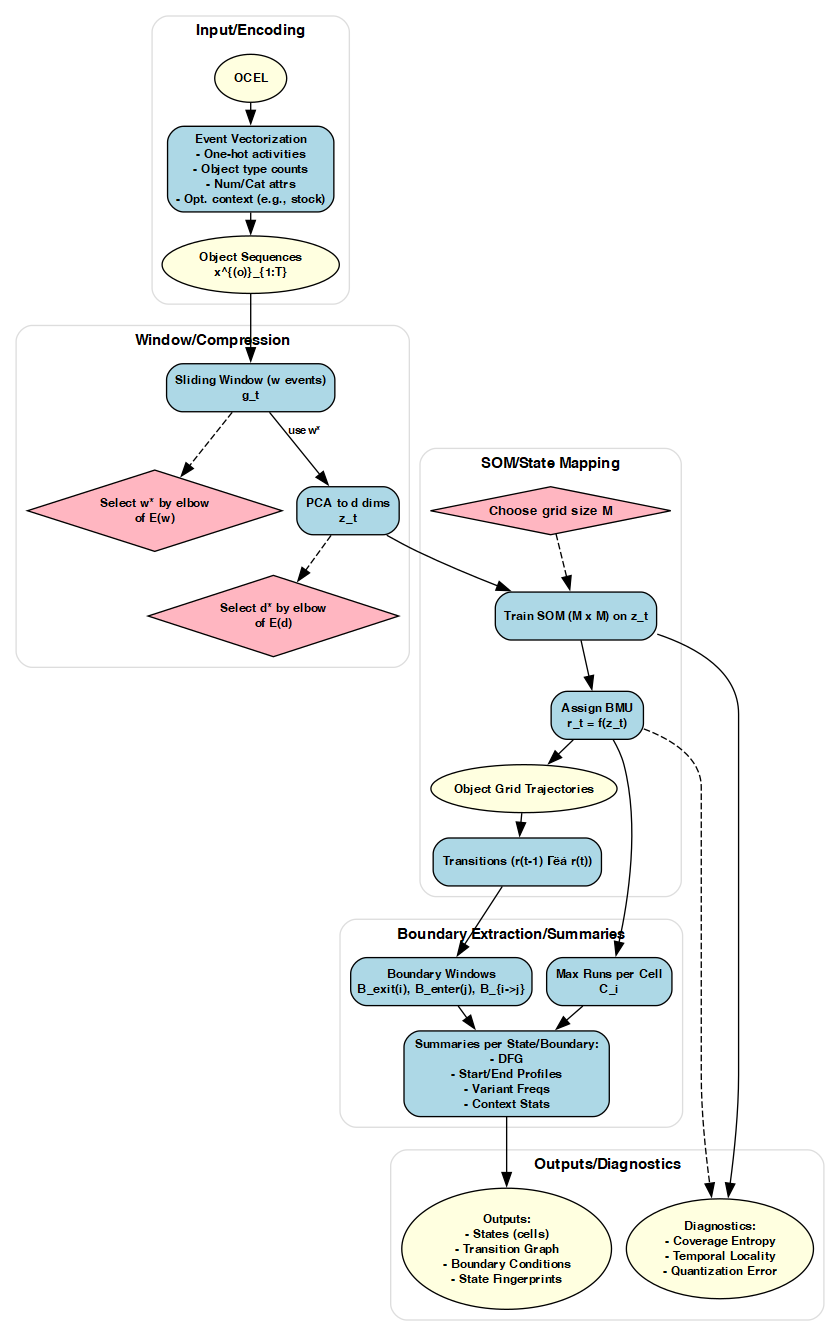
\includegraphics[width=0.74\linewidth]{fig_pipeline.png}
\caption{Pipeline from the base paper: window, compress, map, then summarize states and boundaries. Extracted from the paper PDF.}
\label{fig:pipeline}
\end{figure}

\section{Sliding Windows}

\Task{Window definitions}
For an object $o$ with ordered vectors $x_{1:T}^{(o)}$, the paper uses the trailing concatenation window
\[
g_t^{(o)}=\left[x_{t-w+1}^{(o)}\middle|x_{t-w+2}^{(o)}\middle|\cdots\middle|x_t^{(o)}\right]\in\R^{wn},\qquad t\geq w.
\]
Write the analogous trailing-window formula for a traditional event log case $c$, using vectors $x_{1:T}^{(c)}$. Then write two short comparison bullets:
\begin{itemize}
\item \textbf{Concatenation:} preserves order and positional information, but grows the dimension to $wn$.
\item \textbf{Mean aggregation:} maps the same window to $\bar{g}_t^{(o)}=\frac{1}{w}\sum_{j=t-w+1}^{t}x_j^{(o)}\in\R^n$, losing within-window order but staying compact.
\end{itemize}
Finish with one concrete thesis scenario where concatenation is preferable and one concrete thesis scenario where mean aggregation is preferable.

\Task{Window computation}
A single object has five events at $t=1,2,3,4,5$ with
\[
x_1=\begin{bmatrix}1\\0\\2\end{bmatrix},\quad
x_2=\begin{bmatrix}0\\1\\1\end{bmatrix},\quad
x_3=\begin{bmatrix}1\\1\\0\end{bmatrix},\quad
x_4=\begin{bmatrix}0\\2\\1\end{bmatrix},\quad
x_5=\begin{bmatrix}2\\0\\1\end{bmatrix}.
\]
\begin{enumerate}[label=(\alph*)]
\item For $w=1,2,3$, list all admissible concatenated vectors $g_t$.
\item For $w=1,2,3$, compute the mean-aggregated versions $\bar{g}_t$.
\item Draw the $w=2$ trailing windows on the timeline below.
\end{enumerate}
\WindowTimeline
\answerspace[1.0cm]

\Task{Window function}
Implement \texttt{compute\_windows(event\_vectors, w)}. It should return concatenated trailing windows for every event position, using a zero vector for missing early context.

\begin{lstlisting}[style=python]
import numpy as np

def compute_windows(event_vectors: np.ndarray, w: int) -> np.ndarray:
    """Return one concatenated trailing window per event.

    Parameters
    ----------
    event_vectors:
        Array of shape (T, n).
    w:
        Number of events per trailing window.

    Returns
    -------
    windows:
        Array of shape (T, w*n). Early windows are left-padded with zeros.
    """
    # TODO: implement
    raise NotImplementedError

X = np.array([[1, 0, 2],
              [0, 1, 1],
              [1, 1, 0],
              [0, 2, 1],
              [2, 0, 1]], dtype=float)

print(compute_windows(X, w=2))
\end{lstlisting}

Test on the hand-computation example above. Print the returned matrix for $w=2$ and verify that the first row is $[0,0,0\mid 1,0,2]$ and the last row is $[0,2,1\mid 2,0,1]$.

\Task{Window-size elbow}
The paper forms candidate window datasets in $\R^{wn}$, applies PCA at a fixed probe dimension, and computes a reconstruction error curve $E(w)$. Provide three answers: describe the elbow point geometrically, state why $E(w)$ usually decreases as $w$ grows, and give one reason why an overly large $w$ can still hurt state discovery.
\answerspace[1.4cm]

\section{PCA -- Compress}

\Task{PCA formulas}
Given centered data $X_c\in\R^{m\times n}$, define
\[
\Sigma=\frac{1}{m}X_c^\top X_c,\qquad
\Sigma v_i=\lambda_i v_i,\quad
\lambda_1\geq\lambda_2\geq\cdots\geq\lambda_n\geq 0,
\]
with orthonormal eigenvectors $v_i$. PCA selects $W=[v_1,\ldots,v_d]$ and maps
\[
z=W^\top(x-\mu),\qquad \hat{x}=\mu+Wz=\mu+WW^\top(x-\mu).
\]
For one point,
\[
e(x)=\|x-\hat{x}\|_2^2,
\]
and for a dataset the average squared reconstruction error is
\[
\frac{1}{m}\sum_{j=1}^{m}\left\|x^{(j)}-\hat{x}^{(j)}\right\|_2^2.
\]
The explained variance ratio is
\[
\operatorname{EVR}(d)=\frac{\sum_{i=1}^{d}\lambda_i}{\sum_{i=1}^{n}\lambda_i}.
\]
After the formulas, write the PCA optimality claim exactly: among all rank-$d$ linear reconstructions, PCA minimizes the average squared reconstruction error. Then add two sentences explaining why this compression step is useful before SOM training.

\Task{PCA by hand}
Use the four centered data points
\[
(-2,-1),\quad (-1,0),\quad (1,0),\quad (2,1).
\]
\begin{enumerate}[label=(\alph*)]
\item Compute the covariance matrix $\Sigma=\frac{1}{4}X^\top X$.
\item Find the eigenvalues and eigenvectors analytically.
\item Project all four points to 1-D along the leading eigenvector $v_1$.
\item Compute $\operatorname{EVR}(1)$.
\item Sketch the points, the $v_1$ direction, and the projection of $(2,1)$.
\end{enumerate}
\answerspace[2.0cm]

\Task{Elbow rule on eigenvalues}
Let the PCA eigenvalues be
\[
\lambda=(9,\;6,\;1,\;0.4,\;0.1).
\]
For $d=1,\ldots,4$, compute residual variance
\[
E(d)=\sum_{i=d+1}^{5}\lambda_i.
\]
Normalize the curve using the paper's rule
\[
\tilde{d}=\frac{d-1}{d_{\max}-1},\qquad
\tilde{E}(d)=\frac{E(d)-E(d_{\max})}{E(1)-E(d_{\max})}.
\]
The reference line from $(0,1)$ to $(1,0)$ is $\tilde{d}+\tilde{E}-1=0$, so select
\[
\hat{d}=\arg\max_d\frac{|\tilde{d}+\tilde{E}(d)-1|}{\sqrt{2}}.
\]
Draw the scree plot and mark the selected $\hat{d}$.
\answerspace[1.8cm]

\Task{PCA implementation}
Implement \texttt{pca\_reduce(X, d)}. Then apply it to a random $50\times 8$ matrix and plot $\operatorname{EVR}(d)$ for $d=1,\ldots,8$.

\begin{lstlisting}[style=python]
import numpy as np
import matplotlib.pyplot as plt

def pca_reduce(X: np.ndarray, d: int):
    """Center X, eigendecompose covariance, and return Z plus EVR(d)."""
    # TODO:
    # 1. compute mu and centered Xc
    # 2. compute Sigma = Xc.T @ Xc / len(X)
    # 3. use np.linalg.eigh, sort descending
    # 4. project to top d components
    # 5. return Z, evr
    raise NotImplementedError

rng = np.random.default_rng(7)
X = rng.normal(size=(50, 8))
\end{lstlisting}

Report the returned shape of $Z$, the EVR for $d=2$, and one sentence comparing the EVR curve with the reconstruction-error intuition from the previous task.

\Task{Intra-case PCA hypothesis}
Write a structured answer with three paragraphs: how intra-case prefix vectors differ from pooled OCEL object windows, whether this should increase or decrease the expected number of PCA components, and which empirical diagnostic you would inspect to confirm the choice of $d$.
\answerspace[1.3cm]

\section{Self-Organizing Maps}

\Task{SOM formulas}
An SOM has prototypes $\{w_i\}_{i=1}^{M_xM_y}$, $w_i\in\R^d$, located at grid coordinates
\[
G=\{(p,q):p=1,\ldots,M_x,\;q=1,\ldots,M_y\}.
\]
For input $z\in\R^d$, the best-matching unit is
\[
b(z)=\arg\min_i\|z-w_i\|_2,\qquad f(z)=r_{b(z)}.
\]
During training, for selected input $z$,
\[
w_i(t+1)=w_i(t)+\eta(t)h_{b,i}(t)(z-w_i(t)),
\]
where
\[
h_{b,i}(t)=\exp\left(-\frac{\|r_b-r_i\|_2^2}{2\sigma(t)^2}\right).
\]
After the update rule, state the topology-preservation property in one precise sentence and state why it makes state trajectories interpretable.

\Task{SOM update}
Use the following grid coordinates and prototypes:
\[
w_{(0,0)}=\begin{bmatrix}0.2\\0.1\end{bmatrix},\quad
w_{(0,1)}=\begin{bmatrix}0.3\\0.9\end{bmatrix},\quad
w_{(1,0)}=\begin{bmatrix}0.9\\0.2\end{bmatrix},\quad
w_{(1,1)}=\begin{bmatrix}0.8\\0.8\end{bmatrix}.
\]
For input $z=(0.8,0.3)^\top$, learning rate $\eta=0.5$, and Gaussian neighborhood $\sigma=1$:
\begin{enumerate}[label=(\alph*)]
\item Compute the Euclidean distance from $z$ to each prototype and find the BMU.
\item Compute $h_{b,i}$ for each neuron using grid distance.
\item Update every prototype with $w_i^+=w_i+\eta h_{b,i}(z-w_i)$.
\item Plot old and new prototype positions in the 2-D input space.
\end{enumerate}
\answerspace[1.8cm]

\Task{Grid-size score}
For $M=2$ and $M=3$, use the occupancy counts below. Let $N$ be total assigned points, $p_i=n_i/N$,
\[
H(M)=-\sum_i p_i\log p_i,\qquad
\tilde{H}(M)=\frac{H(M)}{\log(M^2)}.
\]
The neighbor-preservation rates are given as $R(2)=0.92$ and $R(3)=0.81$. Compute
\[
J(M)=\alpha\tilde{H}(M)+(1-\alpha)R(M),\qquad \alpha=0.5.
\]
Which $M$ wins?

\begin{center}
\small
\begin{tabular}{c l}
\toprule
Grid & Occupancy counts\\
\midrule
$M=2$ & $(35,30,25,10)$\\
$M=3$ & $(18,15,13,12,11,10,9,7,5)$\\
\bottomrule
\end{tabular}
\end{center}
\answerspace[1.5cm]

\Task{SOM training plot}
Train a $3\times3$ SOM on 100 random 3-D points. Use \texttt{minisom} if installed; otherwise implement the BMU and update rule manually.
\begin{enumerate}[label=(\alph*)]
\item Plot a U-matrix heatmap: each cell's average prototype distance to neighboring cells.
\item Plot the trajectory of 10 sequential points on the grid.
\item Save both plots and note whether adjacent time points tend to remain close.
\end{enumerate}
\begin{lstlisting}[style=python]
rng = np.random.default_rng(12)
X = rng.normal(size=(100, 3))

# TODO: train a 3x3 SOM and compute bmu positions:
# bmus = [(row, col), ...]
\end{lstlisting}

\Task{SOM transition graph}
Using Figure~\ref{fig:somtransition}, write four short answers:
\begin{itemize}
\item Which cells look most stable, based on self-loops or large assigned-window counts?
\item Which transitions appear most frequent?
\item What would a boundary condition look like on this graph?
\item Use the blank grid to sketch a simplified version of the most important transitions.
\end{itemize}
\BlankSOMGrid
\answerspace[0.8cm]

\begin{figure}[htbp]
\centering
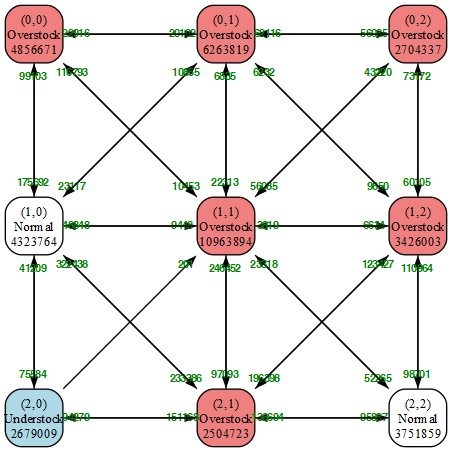
\includegraphics[width=0.58\linewidth]{fig_som_transition.png}
\caption{State-transition view of the paper's $3\times3$ SOM. Extracted from the paper PDF.}
\label{fig:somtransition}
\end{figure}

\section{Boundary Conditions}

\Task{Boundary notation}
For trained SOM states $r_t^{(o)}=f(z_t^{(o)})$, define a transition at $(o,t)$ whenever $r_{t-1}^{(o)}\neq r_t^{(o)}$. The corresponding boundary window is
\[
g_t^{(o)}=(e_{t-w^\star+1}^{(o)},\ldots,e_t^{(o)}).
\]
Boundary collections are updated as
\[
\text{if }r_{t-1}^{(o)}=i,\ r_t^{(o)}=j\neq i,\quad
B_i^{\mathrm{exit}}\leftarrow B_i^{\mathrm{exit}}\cup\{g_t^{(o)}\},\quad
B_j^{\mathrm{enter}}\leftarrow B_j^{\mathrm{enter}}\cup\{g_t^{(o)}\}.
\]
Within-state behavior for state $i$ is collected from maximal intervals
\[
I_i^{(o)}=\{[a,b]:w^\star\leq a\leq b\leq T^{(o)},\; r_t^{(o)}=i\ \forall t\in[a,b],
\ r_{a-1}^{(o)}\neq i,\ r_{b+1}^{(o)}\neq i\ \text{when defined}\}.
\]
Then $C_i$ contains the event-identifier sequences wholly inside state $i$. State exactly what evidence goes into $C_i$, $B_i^{\mathrm{exit}}$, $B_j^{\mathrm{enter}}$, and $B_{i\to j}$. Finish with two sentences describing what differences between these collections reveal.

\Task{Boundary windows in a toy trajectory}
Given state trajectory
\[
\langle A,A,A,B,B,A,A,C\rangle
\]
and event features:

\begin{center}
\small
\begin{tabular}{c c c c}
\toprule
$t$ & State & Activity & Feature note\\
\midrule
1 & A & Submit & normal arrival\\
2 & A & Check & waiting low\\
3 & A & Rework & defect found\\
4 & B & Rework & defect persists\\
5 & B & Approve & manager intervention\\
6 & A & Check & returned to normal\\
7 & A & Approve & cleared\\
8 & C & Escalate & service-level risk\\
\bottomrule
\end{tabular}
\end{center}

\begin{enumerate}[label=(\alph*)]
\item List all transition points.
\item For horizon $h=1$, list the boundary windows around each transition, using one event before and one event after the boundary when available.
\item For the $A\to B$ transition, compare boundary windows against intra-state $A$ windows. Which activity is most enriched near the boundary?
\end{enumerate}
\answerspace[1.5cm]

\Task{Resource-state boundaries}
Define at least three resource-boundary summaries for the thesis. For each summary, specify the input data, the formula or counting rule, and what a high value means at the boundary of a resource-state transition. Consider active cases per resource, handover patterns, queue length, waiting time, activity specialization, and sudden disappearance or replacement of a resource.
\answerspace[1.2cm]

\section{Three State Types for Traditional Event Logs}

\begin{figure}[htbp]
\centering
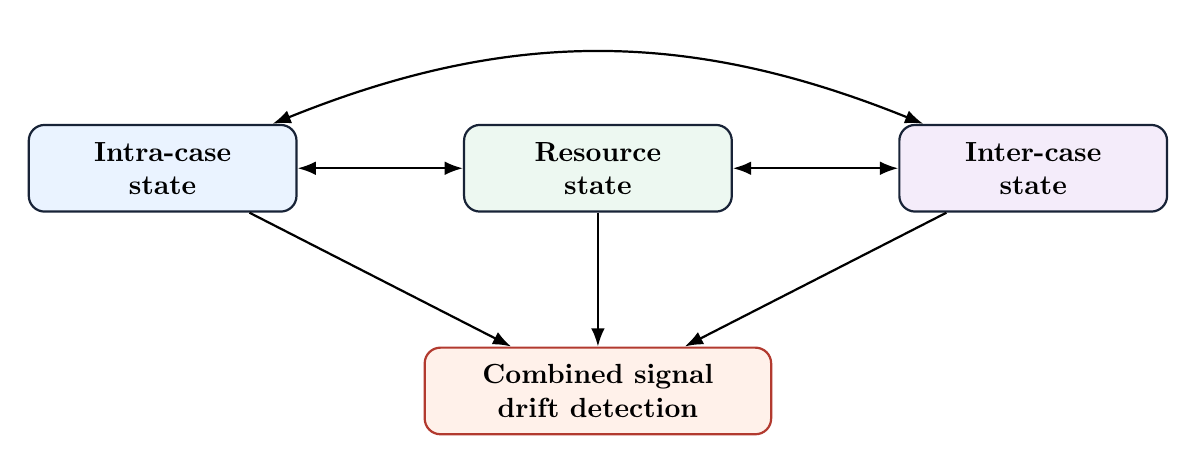
\begin{tikzpicture}[node distance=2.1cm,>=Latex,thick]
  \tikzstyle{stateNode}=[draw=deepnavy,fill=conceptBack,rounded corners=2mm,minimum width=3.4cm,minimum height=1.1cm,align=center,font=\bfseries]
  \node[stateNode] (intra) {Intra-case\\state};
  \node[stateNode,right=of intra,fill=paperBack] (res) {Resource\\state};
  \node[stateNode,right=of res,fill=researchBack] (inter) {Inter-case\\state};
  \node[draw=driftFrame,fill=driftBack,rounded corners=2mm,below=1.7cm of res,minimum width=4.4cm,minimum height=1.1cm,align=center,font=\bfseries] (drift) {Combined signal\\drift detection};
  \draw[<->] (intra) -- (res);
  \draw[<->] (res) -- (inter);
  \draw[<->,bend left=22] (intra) to (inter);
  \draw[->] (intra) -- (drift);
  \draw[->] (res) -- (drift);
  \draw[->] (inter) -- (drift);
\end{tikzpicture}
\caption{Three complementary state views for classical event logs.}
\label{fig:three-states}
\end{figure}

\subsection{Intra-Case State}

\Task{Intra-case definition}
Write the intra-case state definition for event position $t$ of case $c$ as a compact representation of the running prefix $\langle e_1^{(c)},\ldots,e_t^{(c)}\rangle$, mapped through PCA and a SOM to a discrete state:
\[
x_t^{\mathrm{intra}}=\phi_{\mathrm{intra}}(e_1^{(c)},\ldots,e_t^{(c)}),\qquad
s_t^{\mathrm{intra}}=f_{\mathrm{SOM}}^{\mathrm{intra}}(W_{\mathrm{intra}}^\top(x_t^{\mathrm{intra}}-\mu_{\mathrm{intra}})).
\]
After the formula, list the feature vector components you would include:
\begin{itemize}
\item activity one-hot counts in the prefix,
\item time since first event,
\item time since last event,
\item remaining-time estimate,
\item case attributes.
\end{itemize}
Finish with exactly two differences from the paper's per-object OCEL windows.

\Task{Intra-case feature table}
One case has five events:
\[
\begin{array}{rcl}
e_1&=&(\mathrm{Submit},\mathrm{Alice},08{:}00),\\
e_2&=&(\mathrm{Check},\mathrm{Bob},08{:}45),\\
e_3&=&(\mathrm{Approve},\mathrm{Alice},10{:}00),\\
e_4&=&(\mathrm{Notify},\mathrm{Carol},10{:}10),\\
e_5&=&(\mathrm{Close},\mathrm{Bob},11{:}00).
\end{array}
\]
Use activity order
\[
\mathcal{A}=\{\mathrm{Submit},\mathrm{Check},\mathrm{Approve},\mathrm{Notify},\mathrm{Close}\}.
\]
For each event $e_t$, compute:
\begin{enumerate}[label=(\alph*)]
\item prefix activity-count vector over $\mathcal{A}$,
\item elapsed time since first event in minutes,
\item time since last event $\Delta t$ in minutes, using $0$ for the first event,
\item $x_t^{\mathrm{intra}}\in\R^7$ as $[\text{five counts}\mid \text{elapsed}\mid \Delta t]$.
\end{enumerate}

\begin{center}
\scriptsize
\begin{tabularx}{\linewidth}{c l l C{1.3cm} C{1.3cm} Y}
\toprule
$t$ & Activity & Resource & elapsed & $\Delta t$ & $x_t^{\mathrm{intra}}$\\
\midrule
1 & Submit & Alice & & & \\
2 & Check & Bob & & & \\
3 & Approve & Alice & & & \\
4 & Notify & Carol & & & \\
5 & Close & Bob & & & \\
\bottomrule
\end{tabularx}
\end{center}

\Task{Intra-case windows with $w=2$}
Using the five $x_t^{\mathrm{intra}}$ vectors from the previous task, compute concatenated windows
\[
\bar{x}_t^{\mathrm{intra}}=\left[x_{t-1}^{\mathrm{intra}}\middle|x_t^{\mathrm{intra}}\right],
\]
with a zero vector for $t=1$. Which window captures the most activity diversity? Define your criterion explicitly, for example number of nonzero activity-count dimensions across the window.
\answerspace[1.4cm]

\subsection{Resource State}

\Task{Resource-state definition}
Write the resource-state definition at timestamp $\tau$ as a global representation of resource workload and interaction patterns across all cases:
\[
x_\tau^{\mathrm{res}}=\phi_{\mathrm{res}}(L_{\leq \tau},\Delta T),\qquad
s_\tau^{\mathrm{res}}=f_{\mathrm{SOM}}^{\mathrm{res}}(W_{\mathrm{res}}^\top(x_\tau^{\mathrm{res}}-\mu_{\mathrm{res}})).
\]
Then list the candidate features you would compute: workload per resource, active cases per resource, handover frequency, average waiting time, activity distribution per resource, and role assignments. Finish with one concrete resource drift that would not change the activity sequence distribution.

\Task{Resource feature table}
Use this 9-event log:

\begin{center}
\scriptsize
\begin{tabular}{c l l l}
\toprule
CaseID & Activity & Timestamp & Resource\\
\midrule
C1 & Submit & 08:00 & Alice\\
C2 & Submit & 08:05 & Alice\\
C1 & Check & 08:20 & Bob\\
C3 & Submit & 08:25 & Carol\\
C2 & Check & 08:35 & Bob\\
C1 & Approve & 08:50 & Alice\\
C3 & Check & 09:00 & Bob\\
C2 & Approve & 09:10 & Carol\\
C3 & Approve & 09:25 & Carol\\
\bottomrule
\end{tabular}
\end{center}

At $\tau\in\{08{:}20,08{:}35,08{:}50,09{:}10,09{:}25\}$:
\begin{enumerate}[label=(\alph*)]
\item Count active cases per resource. A case is active after its first event and before its final event.
\item Compute handover rate: among consecutive event pairs inside cases observed up to $\tau$, what proportion has a different resource?
\item Build $x_\tau^{\mathrm{res}}=[\mathrm{activeAlice},\mathrm{activeBob},\mathrm{activeCarol},\mathrm{handoverRate}]$.
\item With a global window width $\Delta T=30$ minutes, aggregate resource vectors over $[\tau-\Delta T,\tau]$. Describe how the vector changes when a burst of new cases starts.
\end{enumerate}

\begin{center}
\scriptsize
\begin{tabularx}{\linewidth}{c C{1.4cm} C{1.4cm} C{1.4cm} C{1.5cm} Y}
\toprule
$\tau$ & Alice & Bob & Carol & handover & $x_\tau^{\mathrm{res}}$ after 30-min aggregation\\
\midrule
08:20 & & & & & \\
08:35 & & & & & \\
08:50 & & & & & \\
09:10 & & & & & \\
09:25 & & & & & \\
\bottomrule
\end{tabularx}
\end{center}

\subsection{Inter-Case State}

\Task{Inter-case definition}
Write the inter-case state definition at timestamp $\tau$ as a global temporal behavior representation:
\[
x_\tau^{\mathrm{inter}}=\phi_{\mathrm{inter}}(L_{\leq\tau},\Delta T),\qquad
s_\tau^{\mathrm{inter}}=f_{\mathrm{SOM}}^{\mathrm{inter}}(W_{\mathrm{inter}}^\top(x_\tau^{\mathrm{inter}}-\mu_{\mathrm{inter}})).
\]
Then list the candidate features you would compute: number of active cases, inter-arrival time between new cases, global throughput in events per time unit, and proportion of cases in each current activity. Finish with one example feature pattern for congestion, one for a burst, and one for a slow phase.

\Task{Inter-case feature table}
Using the same 9-event log and timestamps $\tau\in\{08{:}20,08{:}35,08{:}50,09{:}10,09{:}25\}$:
\begin{enumerate}[label=(\alph*)]
\item Count total active cases.
\item Compute the mean inter-arrival gap between case starts up to $\tau$.
\item Compute throughput: number of events in the last 30 minutes.
\item Assemble $x_\tau^{\mathrm{inter}}=[\mathrm{activeCases},\mathrm{meanInterArrivalGap},\mathrm{throughput30min}]$.
\end{enumerate}

\begin{center}
\scriptsize
\begin{tabularx}{\linewidth}{c C{1.6cm} C{2.0cm} C{2.0cm} Y}
\toprule
$\tau$ & active cases & mean inter-arrival gap & throughput & $x_\tau^{\mathrm{inter}}$\\
\midrule
08:20 & & & & \\
08:35 & & & & \\
08:50 & & & & \\
09:10 & & & & \\
09:25 & & & & \\
\bottomrule
\end{tabularx}
\end{center}

\Task{Inter-case SOM assignment}
Assign the five inter-case vectors from the previous task to a $2\times2$ SOM with prototypes:
\[
w_{(0,0)}=(1,20,1),\quad
w_{(0,1)}=(2,15,2),\quad
w_{(1,0)}=(2,10,3),\quad
w_{(1,1)}=(3,8,4).
\]
Scale each feature to comparable units before computing Euclidean distances. For each timestamp, report the closest prototype, draw the resulting grid trajectory, and list the state-transition timestamps. Then give one concrete example from the 9-event log showing how a shared resource or batch-processing constraint appears in the inter-case features.
\answerspace[1.8cm]

\section{Combined State Signal \& Concept Drift Detection}

\Task{Combined state signal}
At each timestamp $\tau$, define the combined state signal as
\[
S_\tau=\left(s_\tau^{\mathrm{intra}},s_\tau^{\mathrm{res}},s_\tau^{\mathrm{inter}}\right).
\]
Give at least three scalar transformations of this triple for drift detection. For each transformation, write either a formula or clear pseudocode:
\begin{itemize}
\item novelty indicator: $1$ if the joint state was rare or unseen in a reference window,
\item distribution distance: total variation, Jensen-Shannon distance, or Earth mover's distance between sliding-window state distributions,
\item trajectory score: distance between mean SOM positions before and after a candidate split,
\item transition intensity: number of state changes per unit time.
\end{itemize}
Choose one scalar for the thesis evaluation and justify the choice in two sentences.

\Task{State-stream drift analysis}
A process runs for 10 timestamps:
\[
\begin{aligned}
s^{\mathrm{intra}}&=\langle A,A,A,A,B,B,B,C,C,C\rangle,\\
s^{\mathrm{res}}&=\langle 1,1,1,2,2,2,2,2,3,3\rangle,\\
s^{\mathrm{inter}}&=\langle \alpha,\alpha,\beta,\beta,\beta,\beta,\gamma,\gamma,\gamma,\gamma\rangle.
\end{aligned}
\]
\begin{enumerate}[label=(\alph*)]
\item At which timestamps does each individual sequence change?
\item Construct the joint sequence $S_\tau$.
\item Plot each sequence on the timeline and mark candidate drift points.
\item At which timestamp does the combined signal most clearly indicate drift?
\end{enumerate}
\DriftTimeline
\answerspace[0.7cm]

\Task{Window distribution shift}
Two time windows yield the following joint-state frequencies:

\begin{center}
\small
\begin{tabular}{l c c}
\toprule
Joint state & $\mathrm{freq}_{W_1}$ & $\mathrm{freq}_{W_2}$\\
\midrule
$(A,1,\alpha)$ & 0.50 & 0.10\\
$(A,2,\beta)$ & 0.25 & 0.20\\
$(B,2,\beta)$ & 0.20 & 0.35\\
$(C,3,\gamma)$ & 0.05 & 0.35\\
\bottomrule
\end{tabular}
\end{center}

\begin{enumerate}[label=(\alph*)]
\item Which state has the largest relative frequency shift?
\item Compute total variation distance:
\[
\operatorname{TV}(P,Q)=\frac{1}{2}\sum_s|P(s)-Q(s)|.
\]
\item Is this sudden or gradual drift? State what additional temporal evidence you would need.
\end{enumerate}
\answerspace[1.1cm]

\Task{SOM trajectory shift}
For 20 events, the state trajectory is
\[
\begin{aligned}
&(0,0),(0,0),(0,1),(0,1),(1,1),(1,1),(1,1),(1,2),(1,2),(1,2),\\
&(2,1),(2,1),(2,2),(2,2),(2,2),(2,2),(2,1),(2,1),(2,0),(2,0).
\end{aligned}
\]
\begin{enumerate}[label=(\alph*)]
\item Draw the trajectory on the $3\times3$ grid.
\item Compute the mean position before and after event 10.
\item Has the center of mass shifted? What process change could this indicate?
\item Define and compute the drift score
\[
\left\|\bar{r}_{\mathrm{before}}-\bar{r}_{\mathrm{after}}\right\|_2.
\]
\end{enumerate}
\BlankSOMGrid
\answerspace[0.7cm]

\Task{Sliding-window distribution detector}
Generate 100 rows with columns \texttt{timestamp}, \texttt{intra\_state}, \texttt{res\_state}, and \texttt{inter\_state}. Inject a known drift at row 50. Then:
\begin{enumerate}[label=(\alph*)]
\item Plot each state stream as a step function.
\item Compute a sliding-window joint-state distribution with window size 10.
\item Flag timestamps where the distribution shift exceeds a threshold.
\end{enumerate}

\begin{lstlisting}[style=python]
from collections import Counter
import numpy as np
import pandas as pd
import matplotlib.pyplot as plt

def state_distribution(states, start, width):
    """Return normalized Counter over states[start:start+width]."""
    # TODO
    raise NotImplementedError

def total_variation(p, q):
    """Compute TV distance between two dict-like distributions."""
    # TODO
    raise NotImplementedError

# TODO: simulate pre-drift and post-drift regimes, then detect row 50.
\end{lstlisting}

\Task{Resource-drift experiment}
Design one experiment showing that the three-SOM signal detects a resource drift that ProDrift or CV4CDD would miss. Specify all four items below:
\begin{itemize}
\item injected drift, such as Bob leaving at time $\tau^\star$ and Dave taking over Bob's checks with longer waiting times,
\item held-constant behavior, such as the same activity sequence distribution before and after drift,
\item evaluation metric, such as detection delay, F1 over drift windows, or localization accuracy,
\item expected outcome for the three-SOM signal versus control-flow-only baselines.
\end{itemize}
\answerspace[1.2cm]

\section{Implementation Roadmap}

\Task{Pipeline skeleton}
Complete the Python skeleton below. Keep the function signatures, replace each placeholder exception with pseudocode-level steps, and write one docstring per function:

\begin{lstlisting}[style=python]
def load_log(path: str):
    """Load a traditional event log as a dataframe with case, activity,
    timestamp, and optional resource/attribute columns."""
    raise NotImplementedError

def encode_events(df, feature_config: dict):
    """Create event-level vectors for intra-case, resource, and inter-case
    feature families."""
    raise NotImplementedError

def compute_windows(event_vectors, w: int, mode: str = "concat"):
    """Build trailing windows using concatenation or aggregation."""
    raise NotImplementedError

def fit_pca(X, d: int):
    """Fit PCA, returning projected vectors plus model parameters."""
    raise NotImplementedError

def fit_som(Z, grid_shape=(3, 3), random_state: int = 0):
    """Train a SOM on PCA vectors."""
    raise NotImplementedError

def assign_states(Z, som):
    """Map each vector to its SOM best-matching unit."""
    raise NotImplementedError

def detect_drift(state_stream, window: int, threshold: float):
    """Compare sliding-window state distributions and return alarms."""
    raise NotImplementedError
\end{lstlisting}

After the code block, add a small table with one row per function: inputs, outputs, and one unit-test idea.

\Task{PM4PY intra-case PCA}
PM4PY's local documentation states that \texttt{tree\_generator.apply()} generates a process tree and that \texttt{process\_tree.playout.apply(tree, parameters=\{"num\_traces": ...\})} performs a process-tree playout returning an event log. Use that API to create a sample log, convert it to a dataframe, compute intra-case feature vectors, and visualize their 2-D PCA projection.

\begin{lstlisting}[style=python]
from pm4py.algo.simulation.tree_generator import algorithm as tree_generator
from pm4py.algo.simulation.playout.process_tree import algorithm as tree_playout
import pm4py

tree = tree_generator.apply(parameters={"mode": 8, "min": 5, "max": 12})
log = tree_playout.apply(tree, parameters={"num_traces": 200})
df = pm4py.convert_to_dataframe(log)

# TODO:
# 1. ensure case/activity/timestamp columns are available
# 2. compute prefix activity-count vectors per case
# 3. append elapsed time and time since previous event
# 4. PCA to 2D
# 5. scatter plot, color by case length bucket
\end{lstlisting}

If the generated playout lacks timestamps, add synthetic timestamps per case before computing temporal features.

\Task{Paper implementation reuse}
Inspect the paper's \href{https://github.com/fit-alessandro-berti/states-detection-understanding}{GitHub repository}. Produce a reuse map with four rows:
\begin{itemize}
\item Which scripts or modules can be reused directly for windowing, PCA, SOM training, state assignment, or visualization?
\item Which parts are OCEL-specific and must be rewritten for traditional event logs?
\item Where should the thesis implementation add resource-state feature builders and inter-case-state feature builders?
\item What tests would demonstrate equivalence to the paper's pipeline on the shared components?
\end{itemize}
\answerspace[1.2cm]

\end{document}
